\documentclass{article}
% Package and macro definitions for CSC 503
% Originally prepared August 23, 2012 by Jon Doyle

%%% Page dimensions
\setlength{\oddsidemargin}{0in}
\setlength{\evensidemargin}{0in}
\setlength{\topmargin}{0in}
\setlength{\textheight}{9in}
\setlength{\textwidth}{6.5in}
\setlength{\headheight}{0in}
\setlength{\headsep}{0in}
\setlength{\footskip}{0.5in}

%%% Font and symbol definition packages
\usepackage{times} 
\usepackage{helvet} 
\usepackage{alltt}
\usepackage{amsfonts, amsmath, amsthm}
\usepackage{amssymb}
\usepackage{stmaryrd}

%%% TikZ diagramming package
\usepackage{tikz}
\usetikzlibrary{arrows,automata}

%%% The modified Sellinger fitch.sty file
\input{fitchhr.sty}

\newcommand{\Z}{\mathbb{Z}}
\newcommand{\Q}{\mathbb{Q}}
\newcommand{\R}{\mathbb{R}}
\newcommand{\N}{\mathbb{N}}
\def\land{\wedge}
\def\lor{\vee}
\def\implies{\rightarrow}
\def\iff{\leftrightarrow}
\def\turn{\vdash}
\def\lrturn{\dashv\vdash}
\def\Cn{\text{Cn}}
\def\Th{\text{Th}}
\def\defeq{\stackrel{\rm def}{=}}

%%% The environment for providing answers to problems
\newenvironment{answer}%
{\par\noindent\textbf{Answer}\par\noindent}%
{}

\def\Sometime{\mathord{\mathsf{F}}}
\def\Forever{\mathord{\mathsf{G}}}
\def\Next{\mathord{\mathsf{O}}}
\def\NextX{\mathord{\mathsf{X}}}
\def\Until{\mathrel{\mathsf{U}}}
\def\Release{\mathrel{\mathsf{R}}}
\def\WeakUntil{\mathrel{\mathsf{W}}}
\def\Before{\mathrel{\mathsf{B}}}

\def\True{\mathord{\mathsf{true}}}

\def\All{\mathord{\mathsf{A}}}
\def\Exists{\mathord{\mathsf{E}}}
\def\Every{\mathord{\mathsf{E}}}

\def\True{\mathord{\mathtt{true}}}
\def\False{\mathord{\mathtt{false}}}

\def\If{\mathrel{\mathtt{if}}}
\def\Else{\mathrel{\mathtt{else}}}
\def\While{\mathrel{\mathtt{while}}}
\def\IfElse#1#2#3{\If #1 \ \{ #2 \} \Else \{ #3 \}}
\def\Whiledo#1#2{\While #1\ \{ #2 \}}
\def\Hcond#1{\llparenthesis #1 \rrparenthesis}
\def\Hoare#1#2#3{\Hcond{#1} \mathrel{#2} \Hcond{#3}}

\def\parmodels{\mathrel{\models_{\textup{par}}}}
\def\totmodels{\mathrel{\models_{\textup{tot}}}}
\def\parturn{\mathrel{\turn_{\textup{par}}}}
\def\totturn{\mathrel{\turn_{\textup{tot}}}}


\def\unityid{rsandil}

\usepackage{amsfonts, amsmath, amsthm}
\usepackage{tikz}
\usetikzlibrary{arrows,automata}

\def\Sometime{\mathord{\mathsf{F}}}
\def\Forever{\mathord{\mathsf{G}}}
\def\Next{\mathord{\mathsf{O}}}
\def\NextX{\mathord{\mathsf{X}}}
\def\Until{\mathrel{\mathsf{U}}}
\def\Release{\mathrel{\mathsf{R}}}
\def\WeakUntil{\mathrel{\mathsf{W}}}
\def\Before{\mathrel{\mathsf{B}}}
\def\True{\mathord{\mathsf{true}}}
\def\All{\mathord{\mathsf{A}}}
\def\Exists{\mathord{\mathsf{E}}}
\def\Every{\mathord{\mathsf{E}}}

\begin{document}
\begin{center}
  {\LARGE CSC 503 Homework Assignment 9}\\[1pc]
  Out: October 12, 2015 \\
  Due: October 19, 2015 \\
  \unityid
\end{center}

Consider the transition model ${\cal M}_1$ depicted in Figure
\ref{f1}.
  \begin{figure}[h]
    \centering
    \caption{Model ${\cal M}_1$}
\begin{center}

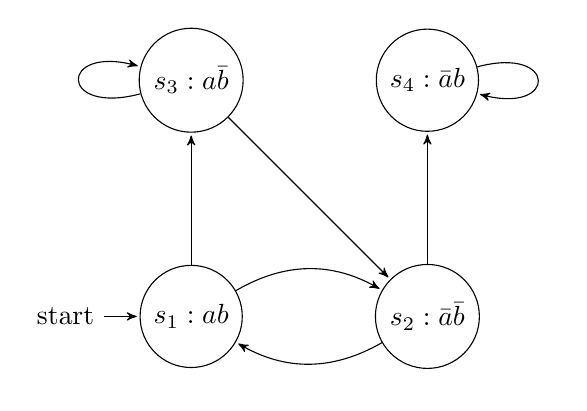
\begin{tikzpicture}[>=stealth',shorten >=1pt,auto,node distance=3cm]
  \node[state] (s3)      {$s_3: a  \bar b$};
  \node[state] (s4)    [right of=s3] {$s_4: \bar a b$};
  \node[initial,state] (s1)   [below of=s3]   {$s_1: a b$};
  \node[state] (s2)   [right of=s1]   {$s_2:   \bar a \bar b$};
  \path[->] 
        (s3) edge         node {} (s2)
        (s3) edge [loop left] node {} (s3)
        (s4) edge [loop right] node {} (s4)
        (s1) edge         node {} (s3)
        (s2) edge         node {} (s4)
        (s1) edge    [bend left] node {} (s2)
        (s2) edge    [bend left] node {} (s1);
\end{tikzpicture}
\end{center}
\label{f1}
\end{figure}
\par
In answering the following questions, recall that all paths are
infinite.  To indicate a path that ends with a repeated set of states,
put parenthesis around the repeated subsequence (e.g.,
$(s_1, s_2)^\infty$.  To indicate a path in which the initial
subsequence $s_1, s_2$ is followed by any possible continuing path,
write ``$s_1, s_2,$ (any)''.

\begin{enumerate}
  \item \textbf{[8 points]} Find a path from the initial state $s_1$
    which satisfies $\Forever a$.
    \begin{answer}
         path which satisfy $\Forever a$. \newline 
    	\textbf{Path}: $s_1-(s_3)^\infty$ \newline
    	\textbf{Explanation}: Starting from state $s_1$ and then repeating on state $s_3$
    	infinitely keeps the literal $a$ always true. Hence this path
    	satisfies $\Forever a$
    \end{answer}

  \item \textbf{[8 points]} Determine whether ${\cal M}_1, s_1 \models
    \Forever a$ and explain why or why not.
        \begin{answer}
    	 ${\cal M}_1, s_1 \models\Forever a$ is False. \newline
    	\textbf{Explanation}:${\cal M}_1, s_1 \models\Forever a$ means that for
    	every path in the model literal '$a$' is always true. This is not the case in
    	the given model. Considering the path $(s_1s_3s_2)^\infty$, which is loop, 
    	we can see that '$a$' is true in all the states but not in $s_2$  	 
    \end{answer}

  \item \textbf{[8 points]} Find a path from the initial state $s_1$
    which satisfies $b \Until a$.
        \begin{answer}
    	There are multiple paths that satisfy $b \Until a$. \newline
    	\textbf{Path}: $s_1-(s_3)^\infty$	\newline
    	\textbf{Explanation}: At first state $s_1$ itself  literal $a$ becomes
    	true. Thus any path starting from state $s_1$ will satisfy the condition $b \Until a$.
    \end{answer}

  \item \textbf{[8 points]} Determine whether ${\cal M}_1, s_1 \models
    b \Until a$ and explain why or why not.
    \begin{answer}
    	${\cal M}_1, s_1 \models b \Until a$ is True and satisfies.	\newline
    	\textbf{Explanation}: For all paths starting from state $s_1$, $b \Until a$
    	is true as in the first state itself we get $a$ as true hence state $s_1$
    	will satisfy the $b \Until a$. Since the condition of $\Until$ is satisfied at the first step itself,
    	we need not check further.
    \end{answer}

  \item \textbf{[8 points]} Find a path from the initial state $s_1$
    which satisfies $\NextX a \Until \NextX (\neg a \land \neg b)$.
    \begin{answer}
    	$\NextX a \Until \NextX (\neg a \land \neg b)$ is satisfied in one of the many
    	paths.	\newline
    	\textbf{Path}: $(s_1-s_2)^\infty$	\newline
    	\textbf{Explanation}: Starting from $s_1$ in the path above $(\neg a \land \neg b)$
    	is true in the next state i.e state $s_2$. since the until condition is satisfied in next step $s_2$, we need not check further. All the path ``$s_1, s_2,$ (any)'' will satisfy $\NextX a \Until \NextX (\neg a \land \neg b)$
    \end{answer}

  \item \textbf{[8 points]} Determine whether
    ${\cal M}_1, s_1 \models \NextX a \Until \NextX (\neg a \land \neg
    b)$ and explain why or why not.
    \begin{answer}
    	${\cal M}_1, s_1 \models \NextX a \Until \NextX (\neg a \land \neg
    b)$ is False.
    	\newline \textbf{Explanation}: Path $s_1-(s_3)^\infty)$  is one such path where ${\cal M}_1, s_1 \models \NextX a \Until \NextX (\neg a \land \neg b)$ does not hold. This is because $s_3$ turns into loop so $ (\neg a \land \neg
    b)$ does not become true  at any further step.
    \end{answer}

  \item \textbf{[8 points]} Find a path from the initial state $s_1$
    which satisfies
    $\NextX (\neg b \land \NextX(\neg a \implies \Forever \neg a))$.
\begin{answer}
    	One of the multiple paths satisfy $\NextX (\neg b \land \NextX(\neg a \implies \Forever \neg a))$.	\newline
    	\textbf{Path}: $s_1-s_2-(s_4)^\infty$.	\newline
    	\textbf{Explanation}: In the path above starting from $s_1$,in the next step i.e $s_2$, $\neg b$ is True. Also  in the next step of $s_2$ i.e $s_4$, $(\neg a \implies \Forever \neg a))$ is  true,thus $\NextX (\neg b \land \NextX(\neg a \implies \Forever \neg a))$ satisfies for above path.
    	
    \end{answer}
  \item \textbf{[8 points]} Determine whether
    ${\cal M}_1, s_1 \models \NextX (\neg b \land \NextX(\neg a \implies
    \Forever \neg a))$ and explain why or why not.
\begin{answer}
    ${\cal M}_1, s_1 \models \NextX (\neg b \land \NextX(\neg a \implies
    \Forever \neg a))$ does not hold.	\newline
    	\textbf{Explanation}: In the path ''$s_1s_3s_2s_1$(any)'' ${\cal M}_1, s_1 \models \NextX (\neg b \land \NextX(\neg a \implies \Forever \neg a))$ does not hold. Since in transition from state $s_2$ to $s_1$ literal $\neg a$ is not true thus $\NextX(\neg a \implies \Forever \neg a))$ will not be true.
    	
    \end{answer}
  \item \textbf{[8 points]} Find a path from the initial state $s_1$
    which satisfies
    $\NextX (\neg a \land \neg b) \land \Sometime (\neg a \land b)$.
        
\begin{answer}
    	Path satisfying above is:
    	\textbf{Path}: $s_1-s_2-(s_4)^\infty$.	\newline
   	
    \end{answer}

  \item \textbf{[8 points]} Determine whether
    ${\cal M}_1, s_1 \models \NextX (\neg a \land \neg b) \land
    \Sometime (\neg a \land b)$ and explain why or why not.
        
\begin{answer}
${\cal M}_1, s_1 \models \NextX (\neg a \land \neg b) \land
    \Sometime (\neg a \land b)$  does not hold. Considering the path $s_1-(s_3)^\infty$, $\neg a \land \neg b$ is never achieved as True. So does not satisfy.
   	
    \end{answer}
%\newpage

\item \textbf{[20 points]} List all subformulas of the LTL formula
  \begin{displaymath}
    ((\neg \NextX p) \WeakUntil q) \Until (\neg p \implies (q \Until
    (\NextX \Forever r \lor \Sometime \NextX \neg q)))
  \end{displaymath}
 \begin{answer} 
 Subformulas are:\newline
 \begin{enumerate}
\item  $((\neg \NextX p) \WeakUntil q) \Until (\neg p \implies (q \Until
    (\NextX \Forever r \lor \Sometime \NextX \neg q)))$  
 \item$((\neg \NextX p) \WeakUntil q)$ 
 \item$\neg \NextX p$
 \item$\NextX p$
 \item$p$
 \item$q$ 
 \item$(\neg p \implies (q \Until(\NextX \Forever r \lor \Sometime \NextX \neg q)))$
 \item$\neg p$
 \item$q \Until(\NextX \Forever r \lor \Sometime \NextX \neg q)$
 \item$(\NextX \Forever r \lor \Sometime \NextX \neg q)$
 \item$\NextX \Forever r$
 \item$\Forever r$ 
 \item$r$ 
 \item$\Sometime\NextX \neg q$
 \item$\NextX \neg q$
 \item$\neg q$
 \end{enumerate}
 
 
  
\end{answer}
\end{enumerate}

\end{document}
